\documentclass[11pt,a4paper]{article}
\usepackage[T1]{fontenc}
\usepackage[utf8]{inputenc}
\usepackage{lmodern}
\usepackage{amsmath,amssymb,amsthm,mathtools,mathrsfs}
\usepackage{graphicx,float,xcolor,multicol}
\usepackage[shortlabels]{enumitem}
\usepackage[margin=27mm]{geometry}
\usepackage{microtype,needspace,placeins}
\usepackage{tikz,tikz-cd}
\usetikzlibrary{arrows.meta,calc,positioning,patterns,decorations.pathreplacing}
\usepackage[colorlinks=true,linkcolor=teal,urlcolor=teal,citecolor=teal]{hyperref}
\setlength{\parindent}{0pt}
\setlength{\parskip}{.6em}
\setcounter{secnumdepth}{0}
\allowdisplaybreaks
\raggedbottom
\providecommand{\cross}{\times}
\DeclareUnicodeCharacter{2020}{\ensuremath{\dagger}}
\DeclareMathOperator{\supp}{supp}
\DeclareMathOperator*{\esssup}{ess\,sup}
\providecommand{\chapter}{\section}
\newenvironment{tool}[2]{\subsection*{Tool #1 --- #2}}{}
\newcommand{\ToolRef}[1]{Tool #1}
\newcommand{\FigureTag}[2]{\textit{Figure #1}}
\newcommand{\Result}[1]{\subsection*{#1}}
\newcommand{\Application}[1]{\subsubsection*{Application\if\relax\detokenize{#1}\relax\else\space--- #1\fi}}
\newcommand{\ProofHeading}{\par\textit{Proof.}\space}
\newcommand{\ProofOf}[1]{\par\textit{Proof of #1.}\space}
\newcommand{\RemarkHeading}{\par\textbf{Remark.}\space}
\newcommand{\NoteHeading}{\par\textbf{Note.}\space}
\newcommand{\ExerciseHeading}{\par\textbf{Exercise.}\space}

% Rendering support only; mathematical text is in each independent post.
\usepackage{booktabs,array,longtable}
\definecolor{HandoutBlue}{HTML}{2F6690}
\definecolor{HandoutNavy}{HTML}{17365D}
\newtheorem{theorem}{Theorem}
\newtheorem{lemma}[theorem]{Lemma}
\newtheorem{proposition}[theorem]{Proposition}
\newtheorem{corollary}[theorem]{Corollary}
\newtheorem{conjecture}[theorem]{Conjecture}
\newtheorem{definition}{Definition}
\newtheorem{example}{Example}
\newtheorem{namedtoolcounter}{Tool}
\newenvironment{namedtool}[1]{\begin{namedtoolcounter}[#1]}{\end{namedtoolcounter}}
\newtheorem*{claim}{Claim}
\newtheorem*{remark}{Remark}
\newtheorem*{exercise}{Exercise}
\newtheorem*{question}{Question}
\newtheorem*{observation}{Observation}
\newcommand{\SourceChapter}[2]{\section*{#2}}
\newcommand{\Lecture}[2]{\section*{Lecture #1: #2}}
\newcommand{\unclear}[1]{\textit{[unclear: #1]}}
\newcommand{\sourcegap}{\textit{[unfinished in the source]}}
\DeclareMathOperator{\dist}{dist}
\DeclareMathOperator{\id}{id}
\DeclareMathOperator{\Hol}{Hol}
\DeclareMathOperator{\Per}{Per}
\DeclareMathOperator{\Fix}{Fix}
\DeclareMathOperator{\diam}{diam}
\DeclareMathOperator{\Var}{Var}
\DeclareMathOperator{\Leb}{Leb}
\DeclareMathOperator{\Hom}{Hom}
\DeclareMathOperator{\End}{End}
\DeclareMathOperator{\Ann}{Ann}
\DeclareMathOperator{\Spec}{Spec}
\DeclareMathOperator{\Max}{Max}
\DeclareMathOperator{\Ob}{Ob}
\DeclareMathOperator{\Tor}{Tor}
\DeclareMathOperator{\Ass}{Ass}
\DeclareMathOperator{\Mor}{Mor}
\DeclareMathOperator{\Fun}{Fun}
\DeclareMathOperator{\Nat}{Nat}
\DeclareMathOperator{\Cone}{Cone}
\DeclareMathOperator{\MCG}{MCG}
\DeclareMathOperator{\Aut}{Aut}
\DeclareMathOperator{\Deck}{Deck}
\DeclareMathOperator{\SL}{SL}
\DeclareMathOperator{\PSL}{PSL}
\DeclareMathOperator{\Area}{Area}
\DeclareMathOperator{\im}{im}
\DeclareMathOperator{\PSh}{PSh}
\newcommand{\CRing}{\mathsf{CRings}}
\newcommand{\AMod}{A\text{-}\mathsf{Mod}}
\newcommand{\Ab}{\mathsf{Ab}}
\newcommand{\Z}{\mathbb Z}
\newcommand{\Q}{\mathbb Q}
\newcommand{\R}{\mathbb R}
\newcommand{\C}{\mathbb C}
\newcommand{\N}{\mathbb N}
\newcommand{\kk}{\mathbb k}
\renewcommand{\aa}{\mathfrak a}
\newcommand{\bb}{\mathfrak b}
\newcommand{\pp}{\mathfrak p}
\newcommand{\qq}{\mathfrak q}
\newcommand{\mm}{\mathfrak m}
\newcommand{\nn}{\mathfrak n}
\newcommand{\rad}{\mathrm r}
\newcommand{\cat}[1]{\mathsf{#1}}
\setcounter{secnumdepth}{0}
\allowdisplaybreaks

\graphicspath{{figures/lemma-book/}}
\begin{document}
\section*{Triangle Inequalities and Trigonometric Substitutions}
% BLOG-CONTENT-BEGIN
\setcounter{theorem}{41}\begin{lemma}[Triangle inequality]
If $ABC$ is a triangle, then $a+b>c$, where $c=\max(a,b,c)$.
\end{lemma}
This elegant inequality has two nontrivial applications.
\paragraph{Classical application.}
Let $A,B$ be two points on the same side of a line $XY$.
Find $M$ on that line such that $AM+MB$ is minimal.
This gives an alternative proof of the law of reflection.
\begin{figure}[H]\centering
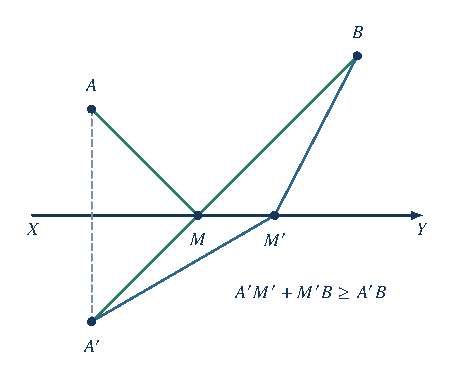
\includegraphics[width=.80\linewidth]{lb1-fig-13.pdf}
\FigureTag{LB1.13}{fig:lb1-13}
\end{figure}
The figure itself is the solution: $A'M'+M'B\geq A'B$.
The geometric interpretation is as follows. Since $AM+MB$ must be the shortest path,
light sent from $A$ to $B$ after reflection must meet the line at the required $M$.
It should satisfy the law of reflection.
Thus choose $M$ so that $\angle AMX=\angle BMY$.

% Source page 19 - left
The second application is the following lemma.
\setcounter{theorem}{42}\begin{lemma}[Triangle-side substitution]
If $a,b,c$ are the sides of a triangle, then there exist positive $x,y,z$
such that $a=x+y$, $b=y+z$, and $c=z+x$.
\end{lemma}
\paragraph{Application.}
For the sides $a,b,c$ of a triangle, prove that $\sum_{\mathrm{cyc}}a(b^2+c^2-a^2)\leq3abc$.
The desired inequality becomes
\begin{align*}
a(b^2+c^2-a^2)+b(c^2+a^2-b^2)+c(a^2+b^2-c^2)&\leq3abc,\\
a^2(b+c-a)+b^2(c+a-b)+c^2(a+b-c)&\leq3abc.
\end{align*}
Substituting gives
\begin{align*}
(x+y)^2(2z)+(y+z)^2(2x)+(z+x)^2(2y)
&\leq3(x+y)(y+z)(z+x),\\
2\bigl((x^2+2xy+y^2)z+(y^2+2yz+z^2)x+(z^2+2zx+x^2)y\bigr)
&\leq3(x+y)(y+z)(z+x),\\
2\bigl(x^2(y+z)+y^2(z+x)+z^2(x+y)+6xyz\bigr)
&\leq3(x+y)(y+z)(z+x),\\
2\bigl((x+y)(y+z)(z+x)+4xyz\bigr)
&\leq3(x+y)(y+z)(z+x).
\end{align*}
This reduces to $8xyz\leq(x+y)(y+z)(z+x)$.
\begin{remark}
The cosine formula also proves the inequality. Put $b^2+c^2-a^2=2bc\cos A$.
Then $\sum_{\mathrm{cyc}}2abc\cos A\leq3abc$ becomes
$\sum_{\mathrm{cyc}}\cos A\leq3/2$, which follows from Jensen's inequality.
This gives a geometric proof.
\end{remark}

These formulas are most useful when understood rather than memorized.
\subsection{Ravi substitution}
$x=s-a$, $y=s-b$, and $z=s-c$, so that
$a=y+z$, $b=z+x$, $c=x+y$, and $s=x+y+z$.
\begin{center}
\renewcommand{\arraystretch}{1.75}
\begin{tabular}{@{}ll@{}}
$s=x+y+z$ &$\displaystyle\sin\frac A2=\sqrt{\frac{(s-b)(s-c)}{bc}}$\\
$\Delta=\sqrt{xyz(x+y+z)}$ &$\displaystyle\sin\frac B2=\sqrt{\frac{(s-c)(s-a)}{ac}}$\\
$\displaystyle r=\sqrt{\frac{xyz}{x+y+z}}$ &$\displaystyle\sin\frac C2=\sqrt{\frac{(s-a)(s-b)}{ab}}$\\
$\displaystyle R=\frac{(x+y)(y+z)(z+x)}{4\sqrt{xyz(x+y+z)}}$ &$\displaystyle\cos\frac A2=\sqrt{\frac{s(s-a)}{bc}}$\\
$\displaystyle r_a=\frac{\sqrt{xyz(x+y+z)}}x$ &$\displaystyle\cos\frac B2=\sqrt{\frac{s(s-b)}{ac}}$\\
$\displaystyle r_b=\frac{\sqrt{xyz(x+y+z)}}y$ &$\displaystyle\cos\frac C2=\sqrt{\frac{s(s-c)}{ba}}$\\
$\displaystyle r_c=\frac{\sqrt{xyz(x+y+z)}}z$ &
\end{tabular}
\end{center}

\paragraph{Two ingenious trigonometric substitutions.}
\[a^2+b^2+c^2\geq4\Delta\sqrt3
\qquad\text{(IMO 1961; Weitzenb\"ock's inequality).}\]
Put $\Delta=\tfrac12 ab\sin C$, so $4\sqrt3\Delta=2\sqrt3ab\sin C$.
The desired inequality is equivalent to
\[\frac ab+\frac ba+\frac{c^2}{ab}\mathrel{\stackrel{?}{\geq}}2\sqrt3\sin C.\]
Apply the cosine rule $c^2=a^2+b^2-2ab\cos C$. Then
\[
\frac{2a}{b}+\frac{2b}{a}\mathrel{\stackrel{?}{\geq}}2(\sqrt3\sin C+\cos C)
\quad\Longrightarrow\quad
\frac{a^2+b^2}{2ab}\mathrel{\stackrel{?}{\geq}}
\sin C\frac{\sqrt3}{2}+\cos C\frac12=\sin(C+30^\circ).
\]
We have $(a^2+b^2)/(2ab)\geq1\geq\sin(C+30^\circ)$. Q.E.D.!
This can also be solved using Ravi substitutions.
\paragraph{Romania (2002).}
If $a,b,c\in(0,1)$, prove that
\[\sqrt{abc}+\sqrt{(1-a)(1-b)(1-c)}<1.\]
Let $a=\cos^2 A$, $b=\cos^2 B$, $c=\cos^2 C$, where
$A,B,C\in(0,\pi/2)$. We have
\[\cos A\cos B\cos C+\sin A\sin B\sin C
<\cos A\cos B+\sin A\sin B=\cos(A-B)\leq1.\]
Q.E.D.!

The following inequality can be proved without Schur's inequality.
For positive reals $a,b,c$, prove that
\[(a+b-c)(b+c-a)(a+c-b)\leq abc.\]
If $a,b,c$ are not the sides of a triangle, the left side is nonpositive and
the result is immediate. Otherwise set $x=a+b-c$, $y=b+c-a$, and $z=a+c-b$.
Then $a=(x+z)/2$, $b=(x+y)/2$, and $c=(y+z)/2$.
The inequality reduces to
\[xyz\mathrel{\stackrel{?}{\leq}}\frac{x+y}{2}\frac{y+z}{2}\frac{z+x}{2},
\qquad (x+y)(y+z)(z+x)\geq8xyz.\]
This completes the proof.
\paragraph{Clever AM--GM.}
If $a,b,c$ are positive reals satisfying $a+b+c=1$, prove that
\[\sqrt{a+bc}+\sqrt{b+ca}+\sqrt{c+ab}\leq2.\]
We cannot do much with the nonhomogeneous expression inside the radical.
Homogenize the expression:
% Source page 49 - right
\[\sqrt{a+bc}=\sqrt{a(a+b+c)+bc}=\sqrt{(a+b)(a+c)}\leq\frac{2a+b+c}{2}.\]
Add the three similar inequalities to obtain
$\sum\sqrt{a+bc}\leq4(a+b+c)/2=2$. Q.E.D.!

\setcounter{theorem}{94}\begin{lemma}[Erd\H{o}s--Mordell inequality]\label{lemma:lb1-97}
Let $P$ be an arbitrary point in or on $\triangle ABC$.
If $p_a,p_b,p_c$ are its distances from the sides, then
\[PA+PB+PC\geq2(p_a+p_b+p_c),\]
with equality if and only if $AB=BC=CA$ and $P$ is the circumcentre.
\end{lemma}
\paragraph{Application: IMO (1991).}
Let $P$ be a point inside $\triangle ABC$.
Prove that at least one of $\angle PAB,\angle PBC,\angle PCA$ is at most $30^\circ$.
\begin{figure}[H]\centering
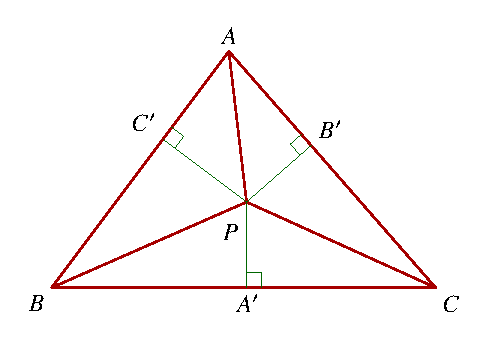
\includegraphics[width=.58\linewidth]{lb1-fig-38.pdf}
\FigureTag{LB1.38}{fig:lb1-38}
\end{figure}
Project $P$ onto $AB,BC,AC$.
We have $PA+PB+PC\geq2(PA'+PB'+PC')$, so at least one of
$PA\geq2PC'$, $PB\geq2PA'$, or $PC\geq2PB'$ holds.
Without loss of generality, take $PA\geq2PC'$.
Then $1/2\geq PC'/PA=\sin\angle PAB$, giving $\angle PAB\leq30^\circ$ or $\angle PAB\geq150^\circ$.
If $\angle PAB\geq150^\circ$, then $\angle PBC<30^\circ$. Q.E.D.!

% Source page 58 - left
\subsection{A trigonometric toolkit}
We begin with a collection of standard trigonometric identities.
\setcounter{theorem}{95}\begin{lemma}[Trigonometric identities]\label{lemma:lb1-98}
\begin{enumerate}
\setcounter{enumi}{0}\item $\sin^2x+\cos^2x=1$.
\setcounter{enumi}{1}\item $1+\cot^2x=\csc^2x$.
\setcounter{enumi}{2}\item $1+\tan^2x=\sec^2x$.
\setcounter{enumi}{3}\item $\sin(a\pm b)=\sin a\cos b\pm\cos a\sin b$.
\setcounter{enumi}{4}\item $\cos(a\pm b)=\cos a\cos b\mp\sin a\sin b$.
\setcounter{enumi}{5}\item $\tan(a\pm b)=(\tan a\pm\tan b)/(1\mp\tan a\tan b)$.
\setcounter{enumi}{6}\item $\sin2a=2\sin a\cos a=2\tan a/(1+\tan^2a)$.
\setcounter{enumi}{7}\item $\cos2a=\cos^2a-\sin^2a=(1-\tan^2a)/(1+\tan^2a)$.
\setcounter{enumi}{8}\item $\sin3a=3\sin a-4\sin^3a$.
\setcounter{enumi}{9}\item $\cos3a=4\cos^3a-3\cos a$.
\setcounter{enumi}{10}\item $|\sin(a/2)|=\sqrt{(1-\cos a)/2}$.
\setcounter{enumi}{11}\item $|\cos(a/2)|=\sqrt{(1+\cos a)/2}$.
\setcounter{enumi}{12}\item $\sin a+\sin b=2\sin((a+b)/2)\cos((a-b)/2)$.
\setcounter{enumi}{13}\item $\cos a+\cos b=2\cos((a+b)/2)\cos((a-b)/2)$.
\setcounter{enumi}{14}\item $\cos a-\cos b=-2\sin((a-b)/2)\sin((a+b)/2)$.
\setcounter{enumi}{15}\item $2\sin a\cos b=\sin(a+b)+\sin(a-b)$.
\setcounter{enumi}{16}\item $2\cos a\cos b=\cos(a+b)+\cos(a-b)$.
\setcounter{enumi}{17}\item $2\sin a\sin b=\cos(a-b)-\cos(a+b)$.
\setcounter{enumi}{18}\item $\cos A=(b^2+c^2-a^2)/(2bc)$.
\setcounter{enumi}{19}\item $a/\sin A=b/\sin B=c/\sin C=2R$.
\end{enumerate}
\end{lemma}
\setcounter{theorem}{96}\begin{lemma}[Trigonometric substitutions and inequalities]\label{lemma:lb1-99}
Here $\alpha,\beta,\gamma\in(0,\pi)$ and
$\alpha+\beta+\gamma=\pi$; the variables in the first three items are positive.
\begin{enumerate}
\setcounter{enumi}{0}\item $ab+bc+ca=1\Longrightarrow a=\tan(\alpha/2),\ b=\tan(\beta/2),\ c=\tan(\gamma/2)$.
\setcounter{enumi}{1}\item $a+b+c=abc\Longrightarrow a=\tan\alpha,\ b=\tan\beta,\ c=\tan\gamma$.
\setcounter{enumi}{2}\item $a^2+b^2+c^2+2abc=1\Longrightarrow a=\sin(\alpha/2),\ b=\sin(\beta/2),\ c=\sin(\gamma/2)$.
\setcounter{enumi}{3}\item $\sin\alpha\sin\beta\sin\gamma\leq3\sqrt3/8$.
\setcounter{enumi}{4}\item $\cos\alpha\cos\beta\cos\gamma\leq1/8$.
\setcounter{enumi}{5}\item $\sin(\alpha/2)\sin(\beta/2)\sin(\gamma/2)\leq1/8$.
\setcounter{enumi}{6}\item $\cos(\alpha/2)\cos(\beta/2)\cos(\gamma/2)\leq3\sqrt3/8$.
\setcounter{enumi}{7}\item $\tan(\alpha/2)+\tan(\beta/2)+\tan(\gamma/2)\geq\sqrt3$.
\end{enumerate}
\end{lemma}
% Source page 58 - right
Let $x,y,z>1$ be real numbers such that $1/x+1/y+1/z=2$.
Prove that $\sqrt{x-1}+\sqrt{y-1}+\sqrt{z-1}\leq\sqrt{x+y+z}$.
Let $x=a+1$, $y=b+1$, and $z=c+1$.
Then $1/(a+1)+1/(b+1)+1/(c+1)=2$, that is, $ab+bc+ca+2abc=1$.
Substitute $ab=\sin^2(\alpha/2)$, $bc=\sin^2(\beta/2)$, and $ac=\sin^2(\gamma/2)$.
We require $\sqrt{ab}+\sqrt{bc}+\sqrt{ca}\leq3/2$, which follows by squaring the original inequality
$\sqrt a+\sqrt b+\sqrt c\leq\sqrt{a+b+c+3}$ and cancelling terms.
It becomes $\sin(\alpha/2)+\sin(\beta/2)+\sin(\gamma/2)\leq3/2$, which follows from Jensen's inequality.
Q.E.D.!
\paragraph{A trigonometric substitution.}
Let $a,b,c$ be positive reals with $a+b+c=1$. Prove that
\[\sqrt{\frac{ab}{c+ab}}+\sqrt{\frac{bc}{a+bc}}+\sqrt{\frac{ca}{b+ca}}\leq\frac32.\]
The substitution gives a two-line solution.
\[\sum_{\mathrm{cyc}}\sqrt{\frac{ab}{c+ab}}
=\sum_{\mathrm{cyc}}\sqrt{\frac{ab}{c(a+b+c)+ab}}
=\sum_{\mathrm{cyc}}\sqrt{\frac{ab}{(c+a)(c+b)}}.\]
We know that $a+b,b+c,c+a$ are the sides of a triangle.
Therefore the last sum is $\sin(\alpha/2)+\sin(\beta/2)+\sin(\gamma/2)\leq3/2$.
Q.E.D.!

\subsection{Two applications}
\paragraph{Problem 2.}
Let the incircle of $\triangle ABC$ touch $BC,AB,CA$ at $D,E,F$, respectively.
If the extension of $DI$ meets $EF$ at $K$, where $I$ is the incentre of $\triangle ABC$,
prove that $A,K,M$ are collinear, where $M$ is the midpoint of $BC$.

It suffices to show that the extension of $AK$ meets $BC$ at $M$, where $BM=MC$.
\begin{figure}[htbp]
\centering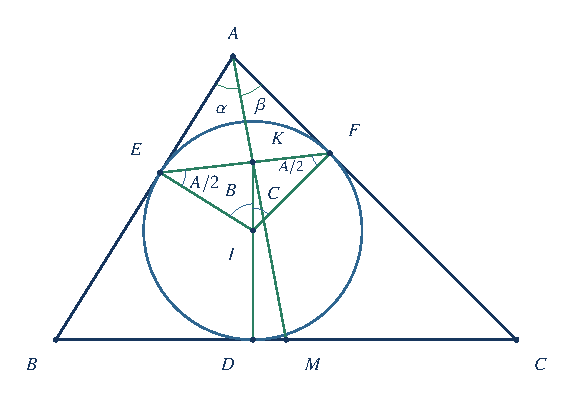
\includegraphics[width=.70\linewidth]{lb1-fig-40.pdf}
\FigureTag{LB1.40}{fig:lb1-40}
\end{figure}
The sine rule for $\triangle FIK$ and $\triangle KIE$ gives
\[
\frac{KE}{\sin B}=\frac{IK}{\sin(A/2)},\qquad
\frac{KF}{\sin C}=\frac{IK}{\sin(A/2)}
\quad\Longrightarrow\quad \frac{KE}{KF}=\frac{\sin B}{\sin C}.
\]
Now apply the sine rule to $\triangle AFK$ and $\triangle AKE$ to obtain
\[
\frac{KE}{\sin\alpha}=\frac{AE}{\sin\angle AKE},\qquad
\frac{KF}{\sin\beta}=\frac{AF}{\sin\angle AKF}
\quad\Longrightarrow\quad
\frac{KE}{KF}=\frac{\sin\alpha}{\sin\beta}.
\]
Thus $\sin\alpha/\sin\beta=\sin B/\sin C$. Applying the sine rule again to
$\triangle ABC$ gives
\[
\frac{AB}{\sin C}=\frac{AC}{\sin B}
\quad\Longrightarrow\quad
\frac{AB}{AC}=\frac{\sin C}{\sin B}=\frac{\sin\beta}{\sin\alpha}.
\]
Now we get $AB\sin\alpha=AC\sin\beta$, and hence
$\frac12 AB\sin\alpha\cdot AM=\frac12 AC\sin\beta\cdot AM$.
This implies $[ABM]=[ACM]\Rightarrow BM=MC$.

\paragraph{Ingenious trigonometric substitution.}
Let $x,y,z>0$ satisfy $xy+yz+zx=3xyz$. Prove $(2y+2z+x)^2>12xyz$.
% Source page 4 - right
From the condition,
$1/(3x)+1/(3y)+1/(3z)=1$, hence $1/(3x)+(y+z)/(3yz)=1$.
Put $1/(3x)=\cos^2\theta$ and $(y+z)/(3yz)=\sin^2\theta$.
Then $\cos\theta=1/\sqrt{3x}$ and $\sin\theta=\sqrt{(y+z)/(3yz)}$.
Using $\sin\theta+\cos\theta>1$, we obtain
\begin{align*}
\frac1{\sqrt{3x}}+\frac{\sqrt{y+z}}{\sqrt{3yz}}>1
&\Longrightarrow \sqrt{3yz}+\sqrt{3x(y+z)}>3\sqrt{xyz}\\
&\Longrightarrow\sqrt{yz}+\sqrt{x(y+z)}>\sqrt{3xyz}.
\end{align*}
Since $\sqrt{yz}\leq(y+z)/2$ and $\sqrt{x(y+z)}\leq(x+y+z)/2$,
we get $y+z+x/2>\sqrt{3xyz}$, proving the result.

\paragraph{APMO (1996).}
For the side lengths $a,b,c$ of a triangle, prove
$\sqrt{a+b-c}+\sqrt{b+c-a}+\sqrt{c+a-b}\leq\sqrt a+\sqrt b+\sqrt c$.

% Source page 17 - left
Write the left-hand side as
$\sum_{\mathrm{cyc}}(\sqrt{c+a-b}+\sqrt{a+b-c})/2$.
Now use $(\sqrt x+\sqrt y)/2\leq\sqrt{(x+y)/2}$ to obtain
\[
\frac{\sqrt{c+a-b}+\sqrt{a+b-c}}2\leq\sqrt a,\qquad
\frac{\sqrt{a+b-c}+\sqrt{b+c-a}}2\leq\sqrt b,\qquad
\frac{\sqrt{b+c-a}+\sqrt{c+a-b}}2\leq\sqrt c.
\]
Adding these three inequalities proves the result.
% BLOG-CONTENT-END
\end{document}
